\chapter{Time Series. Properties and analysis}

\hypertarget{ch2}{This} chapter introduces the basic theory required for an understanding of time series, their properties, and the analysis approach. There also will be explained concepts like stochastic processes, mean value, variance, covariance, autocorrelation (ACF) and partial autocorrelation (PACF) functions, and time series decomposition. 

All the definitions without specific source mention are common for this field of statistics and can be found in many books (Cryer et al. \cite{cryer2008time}, Shumway et al. \cite{shumway2011}). 

\section{Time series and their basic analysis}
First of all, the formal definition of time series needs to be introduced. 
\begin{definition}[\textbf{Time series} \cite{Hyndman2018}]
\textit{Let $T$ be a set of time indices. The time series $Y$ is a sequence of numerical measurements taken at time steps $t \in T$. Formally: $Y = \left\{Y_{t}\;|\;t \in T\right\}$.
}
\end{definition}

In this thesis is considered that time is discrete, all time steps with neighboring indices are equidistant, so we can say, that $t \in Z$. 

\subsection{Goals of time series analysis}

To achieve the best possible results, it is necessary to establish the goals of the time series analysis. They can be formulated as:

\begin{itemize}
    \item \textbf{describing the monitored process} --- identifying the nature of the process represented by the selected time series.
    \item \textbf{forecasting} --- predicting the further development of the process using historical data.
\end{itemize}
\subsection{Real life time series illustrations}

Nowadays, sequentially collected data obtained from some measurements are widespread. There are a lot of different sources of this type of information: business, meteorology, agriculture, epidemiology, and many others.  In this subsection, we show some examples to give a basic idea of what such data looks like and what can be extracted from it.

All time series can be visualized as a graph. On the x-axis there are points in time, on the y-axis there are possible values of measurements taken at a given time.

For an example shown in Figure \ref{fig:daily_inf} we selected a data set that describes the number of people infected daily in the Czech Republic during the pandemic.

At first glance, we can say that this time series has seasonality and growing trend. However, there are different places where the growth rate changes, which may be caused by various cyclic processes, actions of the government, or other reasons.

\begin{figure}[t]
\centering
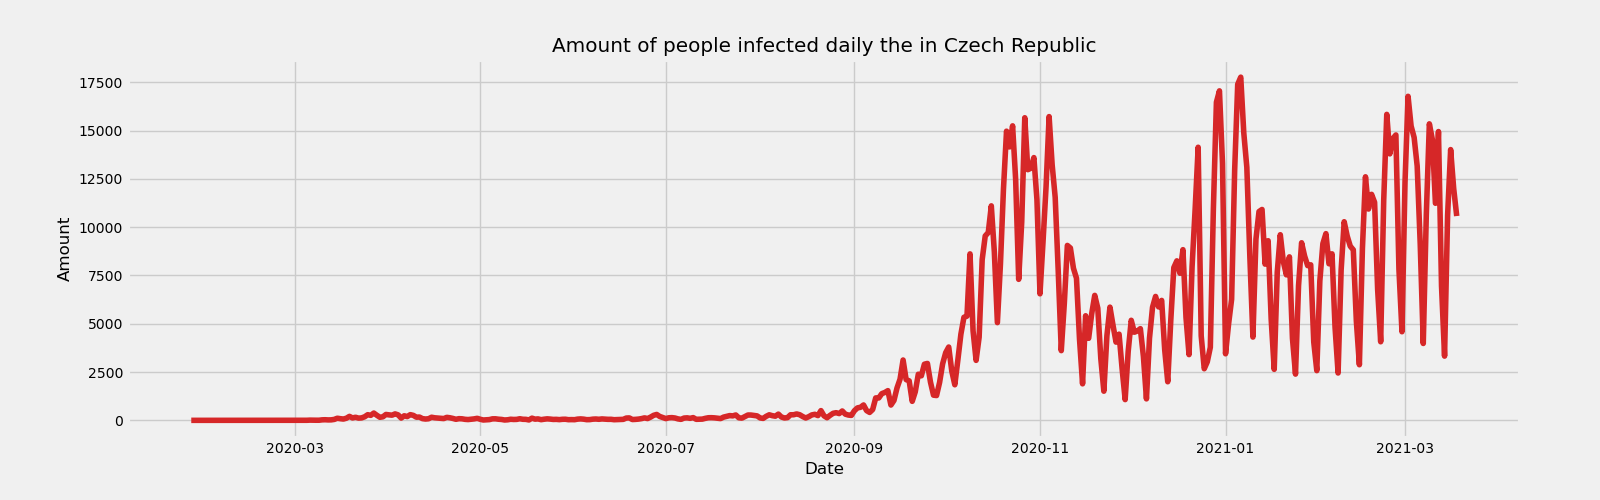
\includegraphics[width=1\textwidth, height=0.5\textwidth]{figures/chapter_02/daily_infected.png}
\caption{Amount of people infected daily in the Czech Republic.}
\label{fig:daily_inf}
\end{figure}

\subsection{Time series decomposition}

To describe the time series demonstrated in Figure \ref{fig:daily_inf_decomposed} it was necessary to use words like \textit{"trend"}, \textit{"seasonality"} and \textit{"cyclic"} \cite{Hyndman2018}. 

\begin{figure}[!ht]
\centering
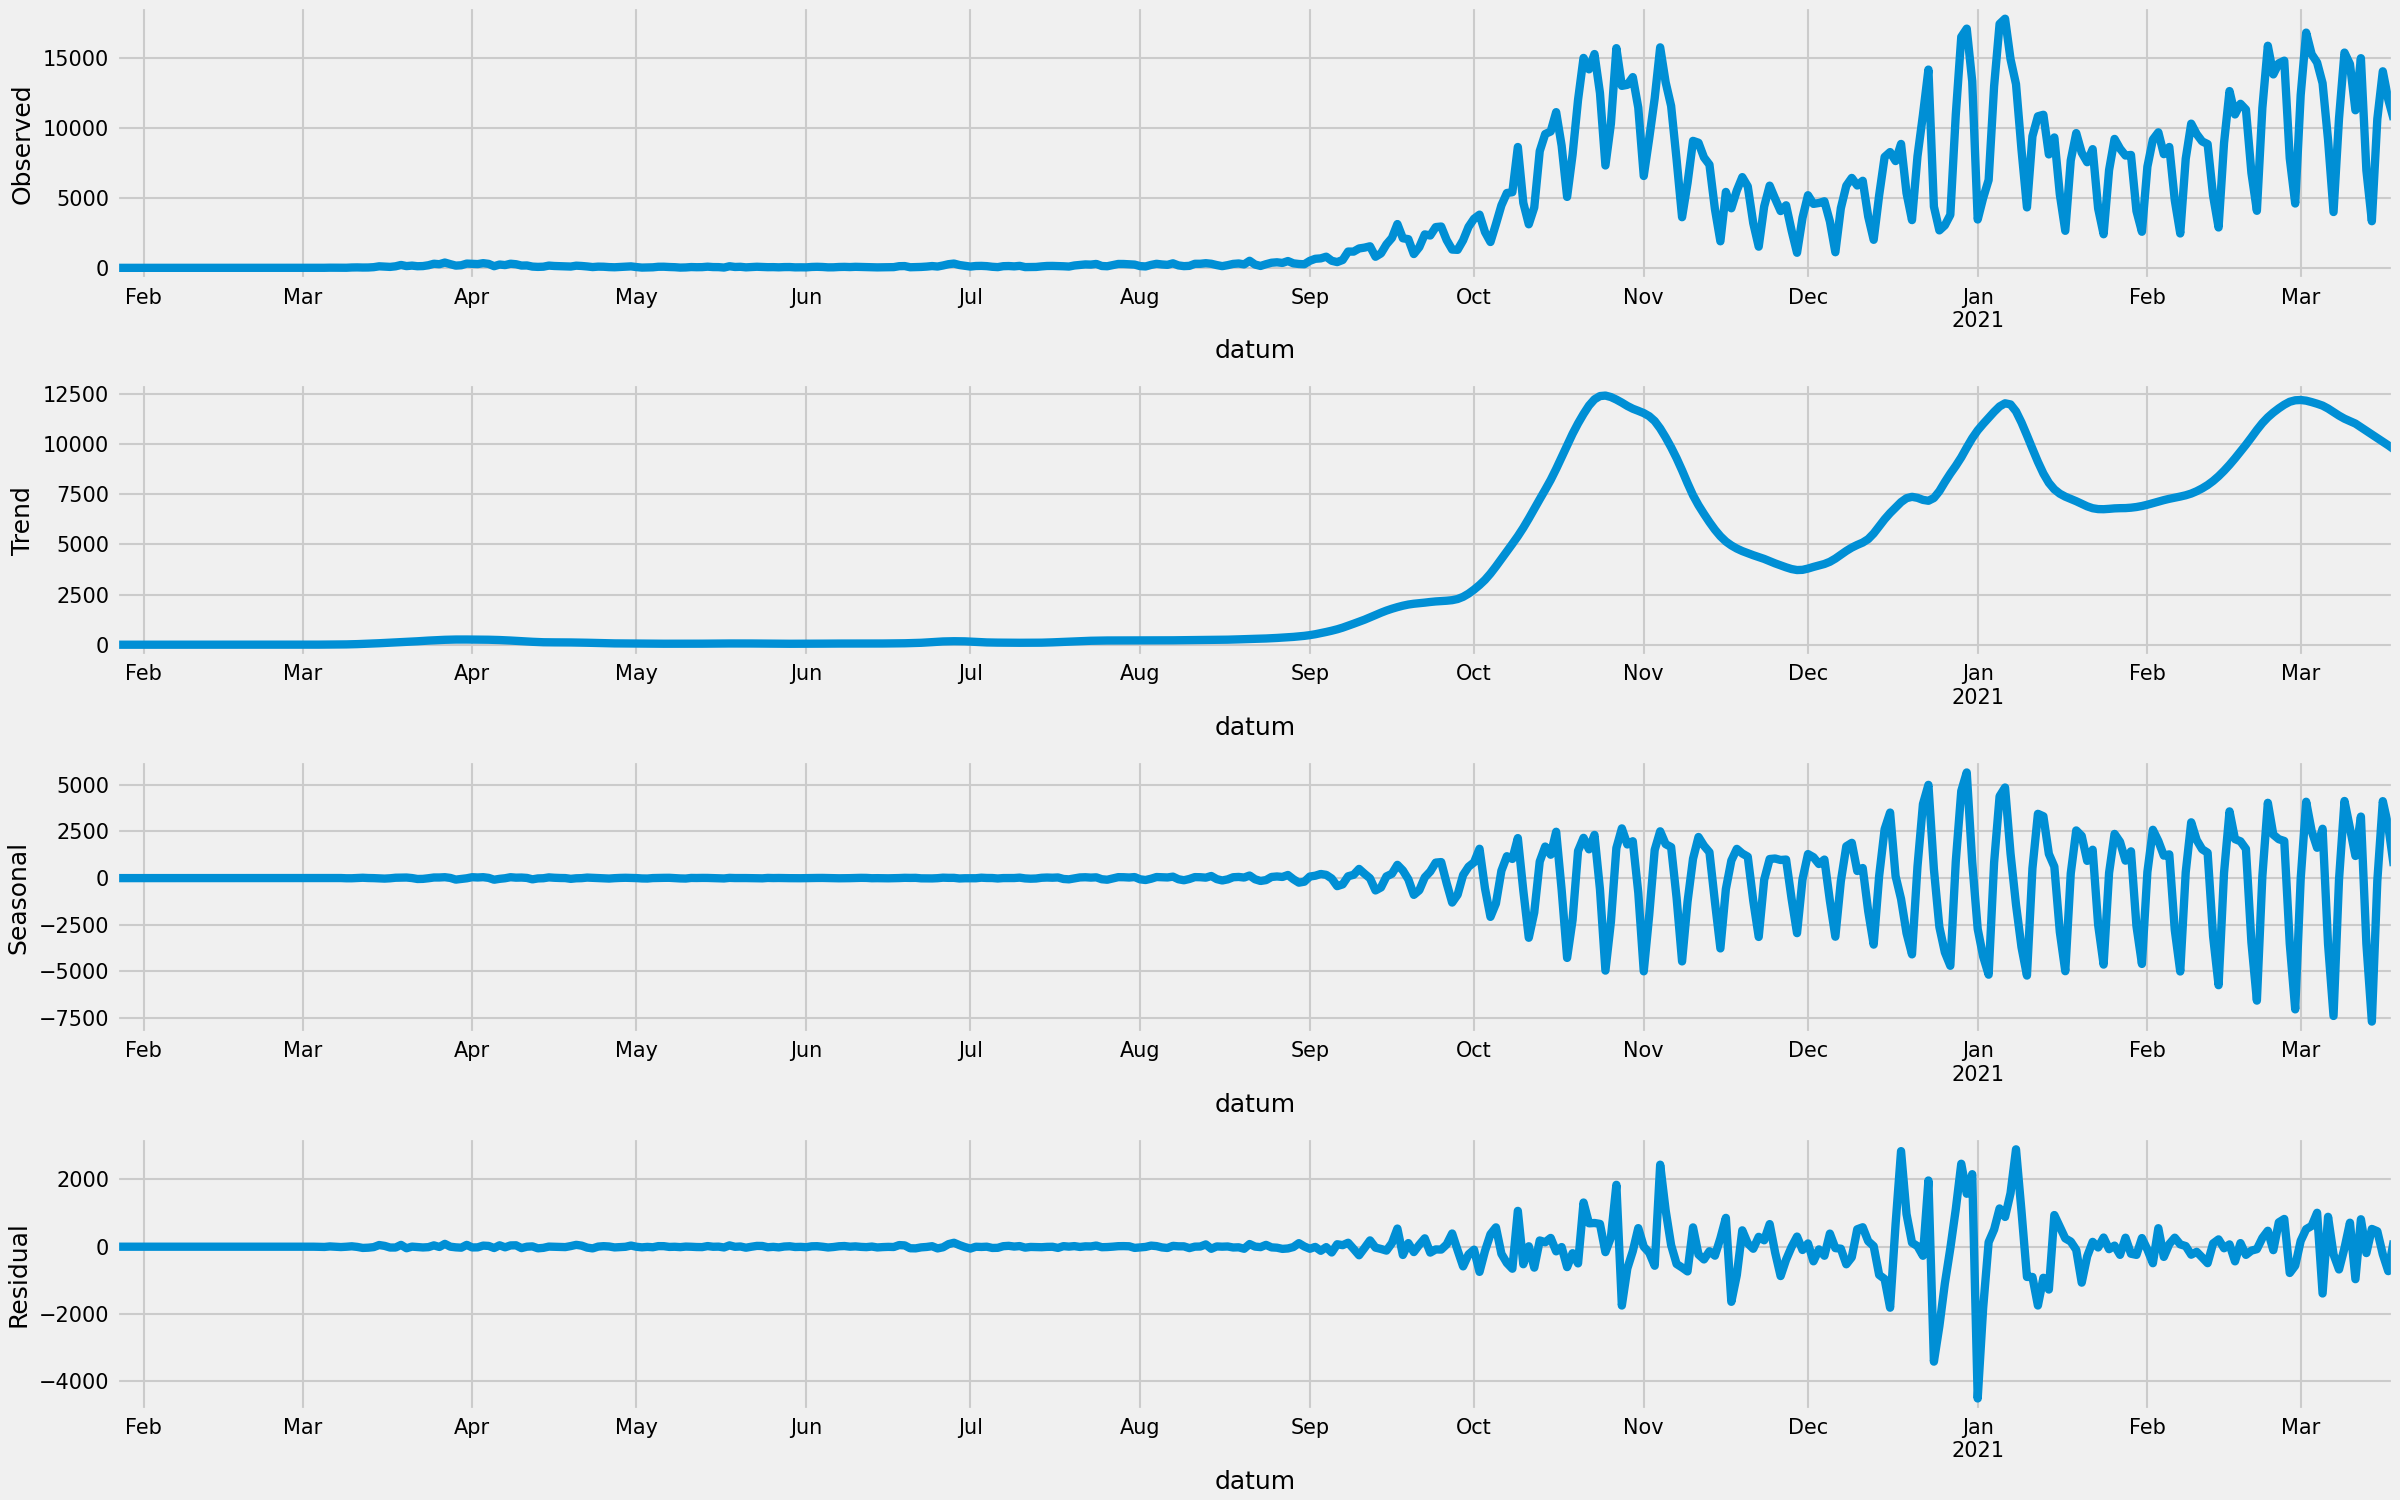
\includegraphics[width=1\textwidth, height=0.9\textwidth]{figures/chapter_02/daily_inf_decomposed.png}
\caption{Daily number of people infected: Decomposition into trend, seasonal, and residual components.}
\label{fig:daily_inf_decomposed}
\end{figure}

It is important to understand that almost all time series can be decomposed into specific parts, that is why we need to introduce a bunch of new definitions.

\begin{definition}[\textbf{Trend}]
\textit{The trend is the component of a time series that represents low frequency variations (long-term increase or decrease of mean value).}
\end{definition}

\begin{definition}[\textbf{Seasonal}]
\textit{The seasonal component represents periodically recurring, relatively regular and predictable (expected) development of the time series. For example, the temperature changes during the year.}
\label{def_seasonal}
\end{definition}

\begin{definition}[\textbf{Cyclic}]
\textit{The cyclic component of a time series represents changes that do not have a specific frequency.}
\end{definition}

Additionally, there are two main models created to describe the time series using these components (seasonal and cyclic components are denoted by one character):
\begin{itemize}
    \item \textbf{additive}:
    \begin{equation}
        Y_t = T_t + S_t + E_t,
    \label{eq_additive_model}
    \end{equation}
    \item \textbf{multiplicative}:
    \begin{equation}
        Y_t = T_t \cdot S_t \cdot E_t,
    \label{eq_multiplicative_model}
    \end{equation}
\end{itemize}
where $Y_t$ is a measured value at time step $t$, $T_t$ --- value of the trend component at the time step $t$, $S_t$ --- value of the seasonal and cyclic components at the time step $t$, $E_t$ --- part of the process at the time step $t$ that cannot be described by other components, also named \textit{residual}.

It is necessary to admit that we can transform the multiplicative model into additive using properties of the logarithm:
\begin{equation}
    \log (T_t \cdot S_t \cdot E_t) = \log T_t + \log S_t + \log E_t.
\end{equation}
Figure \ref{fig:daily_inf_decomposed} demonstrates a time series from the previous section and its decomposition into trend, seasonal, and residual components using the STL model \cite{cleveland1990stl}.

\section{Time series as a stochastic process}

To perform the analysis from the statistical point of view, it is important to understand that time series can be represented as a stochastic process. Therefore, we need to give its definition and describe the basic properties.

\begin{definition}[\textbf{Stochastic process} \cite{cryer2008time}]
\textit{Let $T$ be a set of time indices. Then stochastic process $Y$ is a set defined as $\left\{Y_{t}\;|\;t \in T\right\}$, where $Y_t$ is a random variable.}
\end{definition}
In this work, we will describe this processes in terms of mean value, variance, and covariance.

\subsection{Mean value, Variance, Covariance}

As previously stated, a stochastic process is a set of random variables. In other words, this process has a multivariate distribution and its properties depend on the distribution of each variable considered. Therefore, in this work we will specify terms that can describe this statistical distribution: mean value, variance, and covariance (first and second moments).

\begin{definition}[\textbf{Mean values, Variances, Covariances} \cite{cryer2008time}]
\textit{Let us assume the stochastic process $ Y = \left\{Y_{t}\;|\;t \in T\right\}$, where $T$ is a set of discrete time indices. Then:}
\begin{itemize}
    \item{\textit{\textbf{Mean value function} can be defined as} 
    \begin{equation}
    \mu_{t} = E(Y_{t}), \quad \forall t \in T,
    \label{eq_mean_value}
    \end{equation}}
    \item{\textit{\textbf{Variance} can be defined as 
    \begin{equation}
    \sigma^{2}_{t} = var Y_{t}, \quad \forall t \in T,
    \label{eq_variance}   
    \end{equation}}} 
    \item{\textit{\textbf{Autocovariance function} is specified as} \begin{equation}
    \gamma_{t_1, t_2} = cov(Y_{t_1}, Y_{t_2}), \quad \forall t_1, t_2 \in T,
    \label{eq_autocov_func}
    \end{equation} 
    \textit{where 
    \begin{equation}
    cov(Y_{t_1}, Y_{t_2}) = E[(Y_{t_1} - \mu_{t_1})(Y_{t_2} - \mu_{t_2})].
    \label{eq_covariance}
    \end{equation}}}
\end{itemize}
\end{definition}

\subsection{The Autocorrelation and Partial Autocorrelation functions}

Together with the basic time series moments, we need to introduce the terms of autocorrelation and partial autocorrelation functions. 

In essence, the autocorrelation of time series values denotes the linear (Pearson) correlation coefficient at different time steps. Now, it is important to introduce a more formal definition.

\begin{definition}[\textbf{Autocorrelation function} \cite{cryer2008time}]
\textit{Let us assume atime series $Y = \left\{Y_{t}\;|\; t \in T\right\}$ with mean value $\mu_{t}$ and variance $\sigma_{t}$ for each $t$. The autocorrelation coefficient for time steps $t_1$ and $t_{2}$ is given as}
\begin{equation}
\rho_{t_1, t_2} = corr(Y_{t_1}, Y_{t_2}) = \frac{E[(Y_{t_1} - \mu_{t_1})(Y_{t_2} - \mu_{t_2})]}{\sigma_{t_1}\sigma_{t_2}}, \quad \rho_{t_1, t_2} \in [-1, 1],
\label{eq_autocorrelation_func}
\end{equation}
\textit{on condition, that mean values and variances exist and are positive.}
\end{definition}

It is necessary to understand that its value for nonneighbouring time steps is effected by values of the time series in between. That is why we need to define the partial autocorrelation function, which represents the (auto) correlation of values at timestamps $t_1$ and $t_2$ after removing the effect of the intervening variables.

\begin{definition}[\textbf{Partial autocorrelation function} \cite{cryer2008time}]
\textit{Let us assume a time series $Y = \left\{Y_{t}\;|\; t \in T\right\}$. Then partial autocorrelation coefficient at lag $k$ will be defined as:}
\begin{equation}
\alpha_{t}(k) = corr(Y_{t}, Y_{t-k}\;|\; Y_{t-1}, Y_{t-2}, \ldots, Y_{t-k+1}), \quad \alpha_{t} \in [-1, 1].
\label{eq_partial_autocorrelation_func}
\end{equation}
\end{definition}
These functions can give us an understanding of the repetitive evolution of patterns in the time series. 

\subsection{Stationarity}

During the time series analysis, we might draw conclusions about its structure. Commonly, there are some reasonable simplifications and assumptions about this structure. In this thesis we will use the most important one called \textbf{stationarity}. The basic idea behind this term is that the statistical properties of the process, which generates the time series do not change over time. Specifically, we can highlight \textit{strict} and \textit{weak} stationary time series. 

\begin{definition}[\textbf{Strictly and weakly stationary time series} \cite{box1976time}]
\textit{Let us assume a time series $Y = \left\{Y_{t}\;|\; t \in T\right\}$, we say that this time series is:
\begin{itemize}
    \item \textbf{strictly} stationary if joint distribution of random variables $Y_{t_1}, \ldots, Y_{t_n}$ is equal to joint distribution of $Y_{t_1+\tau}, \ldots, Y_{t_n+\tau}$ for each $t_1, \ldots, t_n$ and $\tau$. 
    \item \textbf{weakly} stationary if it is invariant to time shifts within distribution moments of first and second order. That means:
    \begin{equation}
        E(Y_{t}) = \mu,
    \end{equation}
    and
    \begin{equation}
        cov(Y_{t}, Y_{t+\tau}) = \gamma(\tau),
    \end{equation}
    for each possible $t$ and $\tau$.
\end{itemize}}
\end{definition}

This thesis exploits the weekly stationarity term. Many statistical models used for time series modeling, such as ARMA (introduced in Chapter \hyperlink{ch2}{2}) assume (at least) a weekly stationary process. It is also possible to test the time series on stationarity using different statistical tests. According to Kwiatkowski et al. \cite{KWIATKOWSKI1992159}, it is possible using the combination of \textit{Dickey-Fuller} unit root test and \textit{Kwiatkowski–Phillips–Schmidt–Shin} (KPSS) stationarity test.

Dickey-Fuller test verifies the null hypothesis that the time series has unit roots against the alternative (no unit roots). However, sometimes it may be not enough to exclude, for example, trend-stationarity (stationary process with a trend). KPSS test evaluates the possibility that the time series is trend-stationary (null hypothesis) against the alternative that it is nonstationary. Different combinations of the results of these tests follow the different conclusions specified in Table \ref{tab:stat_tests}. 

\begin{table}[!hbt]
\centering
\resizebox{\textwidth}{!}{%
\begin{tabular}{|l|l|l|}
\hline
\textbf{DF test result} &
  \textbf{KPSS test result} &
  \textbf{Possible conclusion} \\ \hline
rejects null hypothesis &
  \begin{tabular}[c]{@{}l@{}}can not reject null \\ hypothesis\end{tabular} &
  stationarity \\ \hline
\begin{tabular}[c]{@{}l@{}}can not reject null \\ hypothesis\end{tabular} &
  rejects null hypothesis &
  nonstationarity \\ \hline
\begin{tabular}[c]{@{}l@{}}can not reject null \\ hypothesis\end{tabular} &
  \begin{tabular}[c]{@{}l@{}}can not reject null \\ hypothesis\end{tabular} &
  \begin{tabular}[c]{@{}l@{}}not enough data \\ (possible trend-stationarity)\end{tabular} \\ \hline
\begin{tabular}[c]{@{}l@{}}rejects null \\ hypothesis\end{tabular} &
  rejects null hypothesis &
  \begin{tabular}[c]{@{}l@{}}heteroscedasticity,\\ possible structural changes\end{tabular} \\ \hline
\end{tabular}%
}
\caption{Combination of the Dickey-Fuller and KPSS tests with possible conclusion.}
\label{tab:stat_tests}
\end{table}

\subsection{Examples of basic stochastic processes}

For the first example, we decided to select a process named white noise. 
\begin{definition}[\textbf{White noise}]
\textit{White noise is a stochastic process $\left\{ Y_{t}\right\}$, where:
\begin{equation}
E(Y_{t}) = 0,
\end{equation}
\begin{equation}
var(Y_{t}) = \sigma^{2} < \infty,
\end{equation}
\begin{equation}
cov(Y_{t}, Y_{t+\tau}) = \gamma(\tau) = 0.
\end{equation}}
\end{definition}

In other words, it is a process with a constant mean of zero, constant finite variance, and with independent and identically distributed (will be denoted as \textit{i.i.d.}) $Y_{t}$ and $Y_{t+\tau}$ for each possible $t$ and $\tau$. This leads to the conclusion, that this process is also \textit{strictly stationary}.

A special case of the white noise process is a normal (Gaussian) white noise, where $Y_{t} \sim \mathcal{N}(0,\,\sigma^{2})$. The Figure \ref{fig:white_noise} demonstrates an example of a time series generated using this type of process.

For the second example, we will introduce a random walk process. 

\begin{figure}[!htb]
  \centering
  \subfloat[a][Time series generated using the White noise process.]{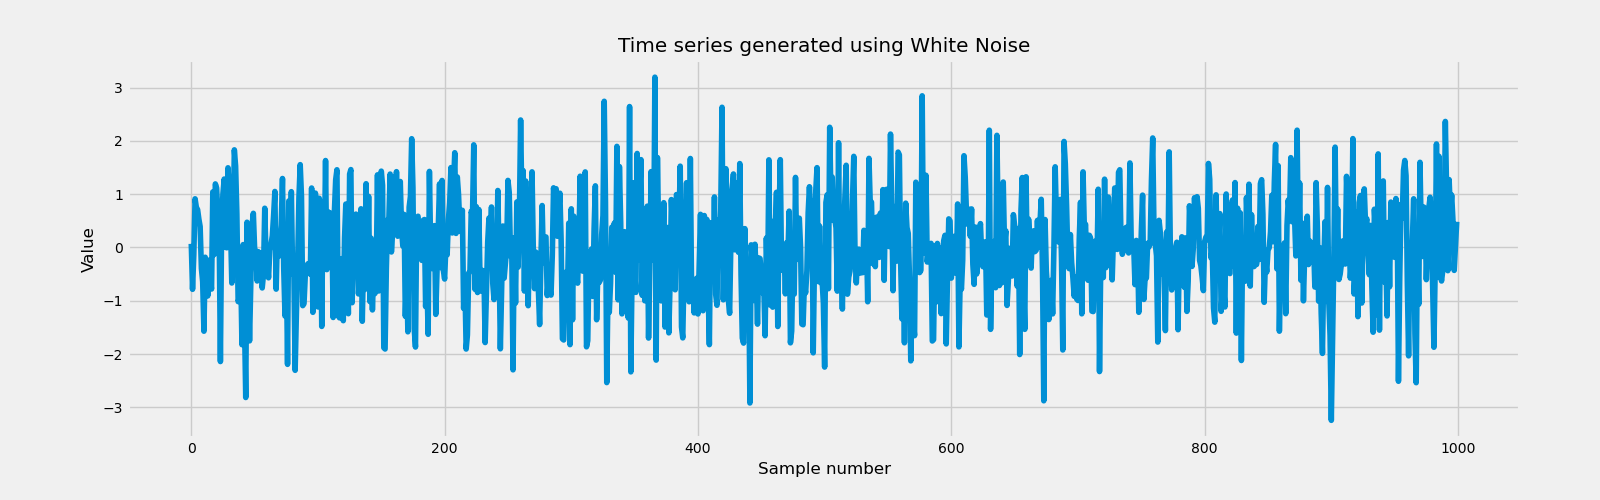
\includegraphics[width=1\textwidth, height=0.4\textwidth]{figures/chapter_02/white_noise.png} 
  \label{fig:white_noise}} \\
  \subfloat[b][Time series generated using the Random walk process.]{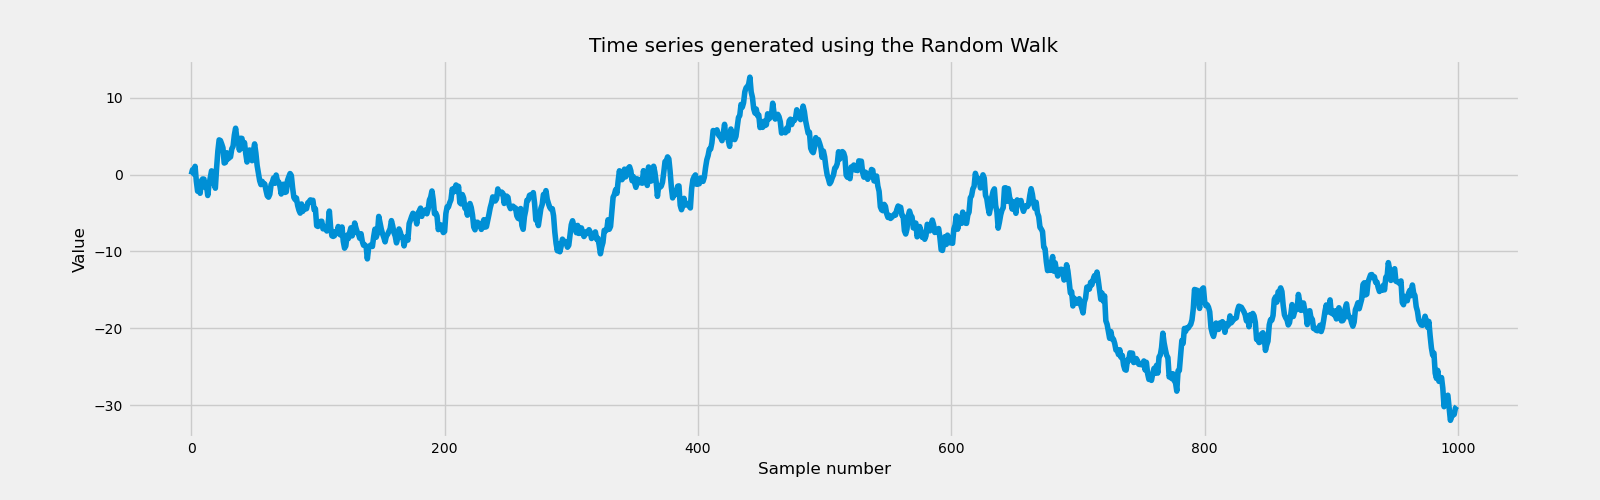
\includegraphics[width=1\textwidth, height=0.4\textwidth]{figures/chapter_02/random_walk.png} 
  \label{fig:random_walk}}
  \caption{Basic stochastic processes examples.} \label{fig:b_ex_ts}
\end{figure}

\begin{definition}[\textbf{Random walk}]
\textit{Let $e_{1}, e_{2}, \ldots$, be a sequence of independent, identically distributed random variables with zero mean value and variance $\sigma^2$ (White noise). Then the stochastic process $\left\{Y_{t}\;|\; t \in T\right\}$ will be a Random Walk if:
\begin{equation}
\begin{aligned}
Y_0 &= 0, \\ 
Y_t &= Y_{t-1} + e_{t},
\end{aligned}
\end{equation}
can also be written as 
\begin{equation}
Y_{t} = \sum_{i=1}^{t} e_i.
\end{equation}}
\label{def_random_walk}
\end{definition}
According to the attributes of the white noise and the properties of mean and variance, we can specify that $Y_t$ has zero mean and variance $t\sigma_{e}^{2}$. Furthermore, the covariance between $Y_{t_1} = \sum_{i=1}^{t_1} e_i$ and $Y_{t_2} = \sum_{i=1}^{t_2} e_i$, where $1 \leq t_1 < t_2$ is $t\sigma_{e}^{2}$. It follows from the covariance property (in the context of white noise):
\begin{equation}
cov(e_{i}, e_{j}) = 
\begin{cases}
    0, & \text{if } i \neq j,\\
    1, & \text{if } i = j.
\end{cases}
\label{eq_cov_white_noise}
\end{equation}
Based on the above, this process is nonstationary. In Figure \ref{fig:random_walk} there can be found an example of a time series generated using the random walk process.  


\section{Summary}
In this chapter, we have introduced the basic concepts behind the term "time series". We have formulated the definition of the time series, its decomposition and explored the representation of time series as a stochastic process. We have also described examples of basic processes that can generate time series.